\relax
\tolerance10000

\item[{\bfseries(I12.3e)}]

(a) $3$ \quad
(b) $\vtor(2,-4,4)$  \quad
(c) 36  \quad
(d) $\vtor(3,-3,3)$  \quad
(e) $\vtor(1,-5,5)$
\bigskip

\item[{\bfseries(I12.4)}]

Every vector is a position vector.  To see of which point it is the position
vector translate it so its initial point is the origin.

Here $\tpv AB = \vek -3\\ 3 \tor$, so $\tpv AB$ is the position vector of
the point $(-3,3)$.
\bigskip

\item[{\bfseries(I12.5)}]

One always labels the vertices of a parallelogram counterclockwise (see
\S\ref{sec:diag-parall}).

$ABCD$ is a parallelogram if $\tpv AB + \tpv AD = \tpv AC$.
$\tpv AB = \vek 1\\ 1 \tor$, $\tpv AC = \vek 2\\ 3 \tor$, $\tpv AD = \vek 3\\
1 \tor$.  So $\tpv AB + \tpv AD \ne \tpv AC$, and $ABCD$ is not a
parallelogram.
\bigskip

\item[{\bfseries(I12.6a)}]

As in the previous problem, we want $\tpv AB + \tpv AD = \tpv AC$.
If $D$ is the point $(d_1, d_2, d_3)$ then
$\tpv AB = \vek 0\\ 1\\1 \tor$,
$\tpv AD = \vek d_1\\ d_2-2 \\ d_3-1\tor$,
$\tpv AC = \vek 4\\ -1\\ 3 \tor$,
so that $\tpv AB + \tpv AD = \tpv AC$ will hold if
$d_1 = 4$, $d_2 = 0$ and $d_3 = 3$.
\bigskip

\item[{\bfseries(I12.6b)}]

Now we want $\tpv AB + \tpv AC = \tpv AD$, so $d_1 = 4$, $d_2 = 2$,
$d_3 = 5$.
\bigskip

\item[{\bfseries(I12.9)}]

Compute the dot product: $\va\dpp\vb = 2s+3(1-s) = 3-s$.  When the
dot-product vanishes the vectors are perpendicular; this happens when
$s=3$.  The angle between the vectors is acute is the dot-product is
positive.  This happens when $3-s>0$, i.e.~when $s<3$.
\bigskip

\item[{\bfseries(I12.11a)}]

The problem is open-ended because it doesn't specify what ``draw'' means.

If you are allowed to use a calculator and a protractor, then you could use the
dot product to compute the angle $\theta$ between the two vectors; then, using
your protractor, draw two line segments that make this angle, and mark off
lengths 3 and 5 to get the vectors.  From the dot-product and the two lengths
you find $3\times5\times\cos\theta = -12$, so $\cos\theta = - \frac{12}{15}=
-0.8$, which implies $\theta = \arccos (-0.8) \approx 2.498\dots$ radians, or
$\theta\approx 143.13\dots$ degrees.

This turns out to be only half the answer:  we have forgotten that the equation
$\cos\theta = -0.8$ has many more solutions than just $\arccos (-0.8)$.  One
other solution is $-\arccos(-0.8)$.  This gives us two vectors $\vb$ with
$\|\vb\|=5$ and $\|\vb\|=5$ and $\va\dpp\vb = -12$.

A different approach goes like this: you could assume $\va=3\ves1$, which has
length 3, and $\vb=\tvek b_1\\b_2\ttor$.  The condition that $\vb$ have length 5
then says $b_1^2 + b_2^2 = 5^2 = 25$, while the dot-product is $\va\dpp\vb =
a_1b_1+a_2b_2 = 3b_1$.  Since the dot-product must be $-12$ we find
$b_1=-\frac{12}{3}=-4$.  Using the length of $\vb$ leads to
$b_2=\sqrt{25-(-4)^2} = \pm3$.  Thus we find two solutions: $\vb = \tvek -4\\
\pm3\ttor = -4\ves1\pm3\ves2$.

You make the drawing.
\bigskip

\item[{\bfseries(I12.11b)}]

No.  The inner product of two vectors is $\va\dpp\vb = \|\va\|\,\|\vb\|
\cos\theta$, and therefore it can never be larger than $\|\va\|\,\|\vb\|$.
\bigskip

\item[{\bfseries(I12.13a)}]

True:
\begin{align*}
  (\va+\vb)\dpp(\va-\vb) &=(\va+\vb) \dpp \va  - (\va+\vb) \dpp\vb\\
  &= \va \dpp \va +\vb \dpp \va  - \va \dpp\vb - \vb \dpp\vb\\
  &= \|\va\|^2 + \| \vb \|^2.
\end{align*}
\bigskip

\item[{\bfseries(I12.13b)}]

True:  This is Pythagoras' theorem.  Here is an algebraic derivation:
\begin{align*}
  \|\va+\vb\|^2 &= (\va+\vb) \dpp (\va+\vb)\\
  &= (\va+\vb) \dpp \va  + (\va+\vb) \dpp\vb\\
  &= \va \dpp \va +\vb \dpp \va  + \va \dpp\vb + \vb \dpp\vb\\
  &= \|\va\|^2 + 2 \va \dpp\vb + \| \vb \|^2\\
  &= \|\va\|^2 + \| \vb \|^2.
\end{align*}
\bigskip

\item[{\bfseries(I12.13c)}]

Not so.
The same computation as for the previous problem shows
\begin{align*}
  \|\va - \vb\|^2 &= (\va-\vb) \dpp (\va-\vb)\\
  &= (\va-\vb) \dpp \va  - (\va-\vb) \dpp\vb\\
  &= \va \dpp \va -\vb \dpp \va  - \va \dpp\vb + \vb \dpp\vb\\
  &= \|\va\|^2 - 2 \va \dpp\vb + \| \vb \|^2\\
  &= \|\va\|^2 + \| \vb \|^2.
\end{align*}
Therefore
\[
\|\va-\vb\|^2 = \|\va\|^2 - \|\vb\|^2
\]
only is true if $\vb=\vvv0$.
\bigskip

\item[{\bfseries(I12.15a)}]

\(  (\va+\vb)\cp(\va+\vb) =\vvv0 \)
\bigskip

\item[{\bfseries(I12.15b)}]

\(  (\va+\vb+\vc)\cp(\va+\vb+\vc) =\vvv0 \)
\bigskip

\item[{\bfseries(I12.15c)}]

\(
    (\va+\vb)\cp(\va-\vb) = 2\va\cp\vb.
\)
\bigskip

\item[{\bfseries(I12.16a)}]

$\va\dpp\vc=\va\dpp(\va\cp\vb) =0$, but for the two given vectors in the problem
$\va\dpp\vc = -1\neq0$, so there cannot be a vector $\vb$ with $\va\cp\vb=\vc$
as $\vc$ is not perpendicular to $\va$.
\bigskip

\item[{\bfseries(I12.16b)}]

In this case $\va\perp\vc$, so the argument from the first part of this problem
doesn't rule out that there might be a solution.  So let's try $\vb =
\tvek b_1\\b_2\\b_3\ttor$.  Then
\[
  \va\cp\vb
  = \vek b_2 \\ -b_1-2b_3 \\ 2b_2\tor \stackrel?= \vc
  = \vek 1\\3\\2\tor.
\]
Solving this for $b_1$, $b_2$, and $b_3$ leads to $b_2=1$, and $-b_1-2b_3=3$ as
only remaining equation.  Since we have found $b_2$ there are still two unknowns
left.  We can choose an arbitrary $b_3$ and set $b_1 = -3-2b_3$, e.g.~$b_3=0$
works, provided we choose $b_1 = -3$.
\bigskip

\item[{\bfseries(II17.7d)}]
 $\kappa(x) = \dfrac{e^x}
{\bigl(1+e^{2x}\bigr)^{3/2}}$.

To find the point with largest curvature:
$\kappa'(t) = \dfrac{e^t} {\bigl(1+e^{2t}\bigr)^{5/2}}
\bigl(1-2e^{2t}\bigr)$, so the maximal curvature (smallest radius of
curvature) occurs when $x=-\frac{1} {2}\ln{2}$.
\bigskip

\item[{\bfseries(III5.1)}]

$-d(x,y)$.
\bigskip

\item[{\bfseries(III5.2)}]

$a<0$, $b>0$, $c>0$.
\bigskip

\item[{\bfseries(III5.3a)}]

$x=-2$ for the $x$-axis, $y=6$ for the $y$-axis, $z=6$ for the $z$-axis.
\bigskip

\item[{\bfseries(III5.3b)}]

$z = 3 - \frac34 x - \frac32y$.
\bigskip

\item[{\bfseries(III5.3c)}]

$\DS \frac{x}{a} + \frac{y}{b} + \frac{z}{c} = 1$ is a nice symmetric way of
writing the equation.
\bigskip

\item[{\bfseries(III5.4)}]

The distance is $\DS \frac{|c|}{\sqrt{1+a^2+b^2}}$.
\bigskip

\item[{\bfseries(III5.5a)}]

This one is already the sum of squares.  We don't have to do anything, and can
immediately conclude that $f(x, y)>0$ for all $(x,y)$ in the plane except the origin,
where $x=y=0$ and $f(x, y) = 0$.
\bigskip

\item[{\bfseries(III5.5b)}]

The square containing $x$ is already complete (no $xy$ terms) and we can immediately
factor $Q(x, y) = (x-y)(x+y)$.
\bigskip

\item[{\bfseries(III5.5c)}]

We complete the square:
\[
  g(x, y) = (x-2y)^2 - y^2.
\]
We get the difference of two squares, so we can factor the quadratic form:
\[
  g(x, y) = (x-2y - y) (x-2y + y) = (x-3y)(x-y).
\]
\bigskip

\item[{\bfseries(III5.5d)}]

This one is positive definite:
\[
  Q
  = 9\bigl( s^2 - 4st + 9 t^2\bigr)
  = 9\bigl[ (s - 2t)^2 -4t^2 + 9 t^2\bigr]
  = 9\bigl[ (s - 2t)^2 + 5 t^2\bigr]
  =9(s-2t)^2 + 45 t^2.
\]
\bigskip

\item[{\bfseries(III5.5e)}]

Positive definite:
\[
  M = \frac12\bigl\{\alpha^2- 2\alpha\beta + 2\beta^2\bigr\}
  =\frac12 \bigl\{(\alpha-\beta)^2 + \beta^2\bigr\}.
\]
\bigskip

\item[{\bfseries(III5.5f)}]

This quadratic form has no $x^2$ term.  When that happens you cna immediately factor
the form, because all terms contain $y$:
\[
Q(x,y) = xy+y^2 = (x+y)y.
\]
This form is indefinite.
\bigskip

\item[{\bfseries(III5.5g)}]

Now this form does have an $x^2$ term, so we \textit{can} complete the square if we
want to \dots but if we look carefully then we see that there's not $y^2$ term.
Because of this we can factor out $x$, and we get
\[
  Q = x^2+2xy = x(x+2y).
\]
The form is indefinite.

What if we don't notice that $y^2$ is missing and just blindly complete the square?
Nothing goes wrong and we get the same answer:
\[
  Q = x^2+2xy = x^2+ 2xy +y^2 - y^2 = (x+y)^2 - y^2 = (x+y - y)(x+y+y) = x(x+2y).
\]
We did work too hard though \verb|:-(|
\bigskip

\item[{\bfseries(III5.6)}]

Complete the square:
\[
  Q=(x+ky)^2 - k^2 y^2 + y^2
   =(x+ky)^2 + (1- k^2) y^2.
\]
If $1-k^2>0$ then we have the sum of two squares.  If $1-k^2<0$, then we can rewrite
$Q$ as the difference of two squares
\[
   Q=(x+ky)^2 - (k^2-1) y^2
   =(x+ky)^2 - \bigl(\sqrt{k^2-1}y\bigr)^2
\]
which is indefinite.  That is all we need to know: we are not actually asked to
factor the form when it is indefinite.  But in case you're wondering, the somewhat
ugly formula is thus:
\[
  Q = \Bigl(x+(k+\sqrt{k^2-1}) y\Bigr) \Bigl(x+(k-\sqrt{k^2-1}) y\Bigr).
\]

The conclusion is that $Q(x,y)$ is positive definite if $-1<k<1$ and indefinite when
$k>1$ or $k<-1$.  In the remaining cases $k=\pm1$ we have
\[
  Q=(x+ky)^2 - k^2 y^2 + y^2
   =(x+ky)^2 + (1- k^2) y^2 = (x\pm y)^2,
\]
i.e.~ the form is a square (it is semidefinite).
\bigskip

\item[{\bfseries(III5.7a)}]

The graph is the saddle surface, the function is defined at all $(x,y)$.  The level
set is given by $xy = c$.  If $c\ne 0$ then this set consists of both branches of the
hyperbola $y=\frac{c}{x}$.  If $c=0$ then $xy=0$ is equivalent with $x=0$ or $y=0$,
so the level set is the union of the $x$-and $y$-axes.
\bigskip

\item[{\bfseries(III5.7b)}]

$z-x^2=0$.
Domain $\R^2$.  Graph is a \emph{parabolic cylinder} and consists of
horizontal lines perpendicular to the $xz$-plane, going through the
parabola $y=x^2$ in that plane.

Level sets: parallel straight lines $x=\pm\sqrt{z}$ if $z>0$,
the $x$ axis if $z=0$, the empty set if $z<0$.
\bigskip

\item[{\bfseries(III5.7c)}]

$z^2-x=0$.
Implicit function.
At least two functions are defined, namely $z=\pm \sqrt{x}$.
Domain: all points $(x,y)$ with $x\ge 0$.
Graph is \emph{half a parabolic cylinder} and consists of
horizontal lines perpendicular to the $xz$-plane, going through the
parabola $z=\sqrt x$ (or $z=-\sqrt x$, depending on which function
you choose) in that plane.

Level sets (assuming we choose the function $z=+\sqrt{x}$):
the line $x=z^2$ if $z\ge0$, empty set otherwise.
\bigskip

\item[{\bfseries(III5.7d)}]

$z-x^2-y^2=0$.
Domain is the whole plane.
Graph is a paraboloid of revolution, obtained by rotating the
parabola $z=x^2$ in the $xz$-plane around the $z$ axis.

Level sets: circle with radius $\sqrt{z}$ for $z>0$,
the origin for $z=0$ (note: this level set is a point rather than a curve),
empty for $z<0$.
\bigskip

\item[{\bfseries(III5.7e)}]

$z^2-x^2-y^2=0$.
Implicit function.  Domain all of $\R^2$.
Possible functions are $z=\pm\sqrt{x^2+y^2}$.
Graph is the cone obtained by rotating the
half line $z=x, x\geq0$ in the $xz$-plane around the $z$ axis
(or the half line $z=-x, x\geq0$, if you chose $z=-\sqrt{x^2+y^2}$.)

Level sets (assuming we choose $z=+\sqrt{x^2+y^2}$):  circle with radius
$z$ when $z>0$, origin when $z=0$, empty when $z<0$.
\bigskip

\item[{\bfseries(III5.7f)}]

$xyz=1$.
Domain the whole plain with the $x$ and $y$-axes removed, i.e.\ all
points $(x, y)$ with $xy\ne0$.
Function is $f(x, y) = \frac{1} {xy}$.
For each $y$ the graph is the hyperbola $z=1/(yx)$ which is just the
standard hyperbola $z=1/x$ stretched vertically by a factor $1/y$.
As $y\to 0$ this factor goes to $\infty$.
\bigskip

\item[{\bfseries(III5.7g)}]

$xy/z^2=1$.
Implicit function.
Domain first and third quadrants (all points with $xy>0$).
Functions $z= \pm \sqrt{xy}$.
Cross sections with planes $y=$constant are half parabolas.

Note: Harder to see, but the surface with equation $xy=z^2$ is in fact
the cone obtained by rotating the $x$-axis around the line
$x=y$ in the $xy$-plane.
\bigskip

\item[{\bfseries(III5.8a)}]

$x>0$.  This one is in the text.
\bigskip

\item[{\bfseries(III5.8b)}]

$x<0$.
\bigskip

\item[{\bfseries(III5.8c)}]

$x>0$.  This is the same region as in part (a):  remember that the polar angle is
only determined up to a multiple of $2\pi$.
\bigskip

\item[{\bfseries(III5.8d)}]

In the upper half plane, $y>0$.
\bigskip

\item[{\bfseries(III5.8e)}]

In the whole plane, except the origin, and the negative $x$-axis.  This formula for
the polar angle $\theta$ clearly is valid in a larger region than the other formulas,
but it does not look half as nice.
\bigskip

\item[{\bfseries(III5.9)}]

The level set for $c=-24$ is the empty set, since it consists of all points on
the lake surface where the lake is $-24$ meters deep--i.e.~where the water
reaches $24$meters {\bfseries\itshape above} the lake.

Similarly, the level set for $c=+400$ is also empty since the lake is not that
deep anywhere.

The level set $d^{-1}(0)$ consists of those points where the lake is $0$meters
deep.  This is exactly the shore line.

The level set $d^{-1}(24)$ consists of all points on the lake surface where the
lake is exactly $24$meters deep.  Form the map it looks like this happens on two
separate curves near the center of the lake.
\bigskip

\item[{\bfseries(III5.10)}]

See \S~\ref{sec:functions-in-PC}.
\bigskip

\item[{\bfseries(III5.11a)}]

The two rectangular strips $-3\leq x\leq3, 2\leq y<\infty$ and
$-3\leq x\leq3, -\infty<y\leq-2$.
\bigskip

\item[{\bfseries(III5.11b)}]

By definition $\arcsin(x)$ is only defined if $-1\leq x\leq1$.
For $\arcsin(x^2+y^2-2)$ to be defined, we must therefore have
$-1\leq x^2+y^2-2 \leq 1$, i.e.\ $1\leq x^2+y^2 \leq 3$.

The domain of this function is
the ring-shaped region between the circles with radii $1$ and
$\sqrt{3}$, both centered at the origin.
Circles are included in the domain.
\bigskip

\item[{\bfseries(III5.11c)}]

The way this function is written both $\sqrt x$ and $\sqrt y$ must be defined,
so the domain consists off all $(x,y)$ with $x\geq0$ and $y\geq0$.
\bigskip

\item[{\bfseries(III5.11d)}]

$\sqrt{xy}$ must exist, which happens for all $(x,y)$ in the first
and third quadrants (axes included.)
\bigskip

\item[{\bfseries(III5.11f)}]

The region in the plane given by $x^2+4y^2\leq16$, which is the region
enclosed by an ellipse with
major axis of length 4, along the $x$ axis, and minor axis of length
2 along the $y$-axis.  The ellipse is included.
\bigskip

\item[{\bfseries(III5.12)}]

The level sets of the function whose graph is a cone are equally spaced circles
(the level set at level $c$ is a circle with radius $c$).  Hence the one on the
right corresponds to the cone, and
the one on the left corresponds to the paraboloid.
\bigskip

\item[{\bfseries(III5.13a)}]

$(0, \frac{1} {2})$ is in the square $Q$, so it is the point closest to
$(0, \frac{1} {2})$.\\
The point $(0,1)$ on the top edge of the square is closest to $(0,2)$.\\
The corner point $(1,1)$ is closest to $(3,4)$.
\bigskip

\item[{\bfseries(III5.13b)}]

$f(0, \frac12) =0 $;
$f(0,2)=1$ and $f(3, 4))=\sqrt{2^2+3^2}=\sqrt{13}$.
\bigskip

\item[{\bfseries(III5.13c)}]

The zero set of $f$ is the square $Q$.
\bigskip

\item[{\bfseries(III5.13d)}]

The level set at level $-1$ is empty.  The others are ``rounded
rectangles,'' see this drawing, in which the square is grey, the dashed
lines are given by $x=\pm1$ or $y=\pm1$.
\begin{center}
    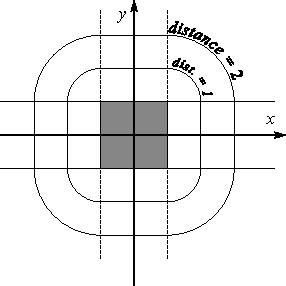
\includegraphics{01distancetosquare.pdf}
\end{center}
\bigskip

\item[{\bfseries(III5.13e)}]

The lines $x=\pm1$ and $y=\pm1$ divide the plane into nine regions.
On each region the function is given by a different formula.
Here they are:
\begin{tabbing}
\=$\boldmath{f(x, y)}$ \=\`\textbf{ if } \ldots \\
\>$0$  \>\` $(x, y)$ in $Q$\\
\>$x-1$ \>\` $x\geq1, |y|\leq 1$\\
\>$y-1$ \>\` $|x|\leq 1, y\geq1$\\
\>$-x-1$ \>\` $x\le-1, |y|\leq 1$\\
\>$-y-1$ \>\` $|x|\leq 1, y\le-1$\\
\>$\sqrt{(x-1)^2+(y-1)^2}$ \>\` $x\ge1$ and $y\ge1$\\
\>$\sqrt{(x-1)^2+(y+1)^2}$ \>\` $x\ge1$ and $y\le-1$\\
\>$\sqrt{(x+1)^2+(y-1)^2}$ \>\` $x\le-1$ and $y\ge1$\\
\>$\sqrt{(x+1)^2+(y+1)^2}$ \>\` $x\le-1$ \& $y\le-1$\\
\end{tabbing}
\bigskip

\item[{\bfseries(III5.14a)}]

At time $t$ we have a line through the origin with slope $\sin t$.
As time progresses this lines turns up and down, and up and down,  etc.
\bigskip

\item[{\bfseries(III5.14b)}]

Same as previous problem, but twice as fast.
\bigskip

\item[{\bfseries(III5.14c)}]

At all times one sees the graph of $y=\sin x$ stretched vertically by a factor $t$.
\bigskip

\item[{\bfseries(III5.14d)}]

Same as previous problem, but twice as fast.
\bigskip

\item[{\bfseries(III5.14e)}]

The graph of $y=\sin 2x$ stretched vertically by a factor $t$.
\bigskip

\item[{\bfseries(III5.14f)}]

Parabola with its minimum on the $x$-axis at $x=t$.
So we see the parabola $y=x^2$ translating from the left to the right
with constant speed 1.
\bigskip

\item[{\bfseries(III5.14g)}]

Parabola with its minimum on the $x$-axis at $x=\sin t$.
So we see the parabola $y=x^2$ translating back and forth horizontally
every $2\pi$ time units.
\bigskip

\item[{\bfseries(III5.14j)}]

At time $t$ we see Agnesi's witch, i.e. the graph $y= a/(1+x^2)$
with amplitude $a=1/(1+t^2)$.  Thus we see a bump whcich starts out small
 at $t=-\infty$, grows to its maximal size at time $t=0$, and then decays
again, until it vanishes at $t=+\infty$.
\bigskip

\item[{\bfseries(III5.16)}]

The graph of $y=g(x-a)$ is obtained from the graph of $y=g(x)$ by
translating the graph of $y=g(x)$ by $a$ units to the right.

Hence the graph of $g(x-ct)$ is the graph of $g(x)$ translated by $ct$
units to the right.  As time changes the graph of $g(x-ct)$ therefore
moves with velocity $c$ to the right.
\bigskip

\item[{\bfseries(III5.17)}]

If you know the graph of a function $y=g(x)$, then you get
the graph of $y=cg(x)$ by stretching the graph of $g$ vertically by
a factor $c$ (here $c$ is a constant.)
If you allow this constant to depend on time, e.g.\ as in this
problem by setting $c=\cos(\omega t)$, then the ``movie'' you get is of a
version of the graph of $g$ which is growing and shrinking vertically.

\begin{center}
    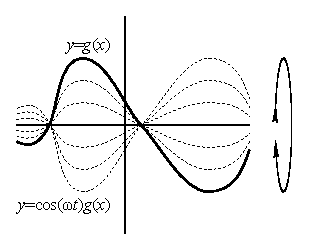
\includegraphics{01standingwave.pdf}
\end{center}
\bigskip

\item[{\bfseries(IV3.2b)}]

$-2xy\sin(x^2y)$, $-x^2\sin(x^2y)+3y^2$
\bigskip

\item[{\bfseries(IV3.2c)}]

$(y^2-x^2y)/(x^2+y)^2$, $x^3/(x^2+y)^2$
\bigskip

\item[{\bfseries(IV3.2g)}]

$2xe^{x^2+y^2}$, $2ye^{x^2+y^2}$
\bigskip

\item[{\bfseries(IV3.2h)}]

$y\ln(xy)+y$, $x\ln(xy)+x$
\bigskip

\item[{\bfseries(IV3.2i)}]

$-x/\sqrt{1-x^2-y^2}$, $-y/\sqrt{1-x^2-y^2}$
\bigskip

\item[{\bfseries(IV3.2l)}]

$\tan y$, $x/\cos^2 y$
\bigskip

\item[{\bfseries(IV3.2m)}]

$-1/(x^2y)$, $-1/(xy^2)$
\bigskip

\item[{\bfseries(IV3.4a)}]

$\DS\pdd\theta x = -\frac{y} {x^2+y^2}$, $\DS\pdd\theta x = \frac{x} {x^2+y^2}$.
\bigskip

\item[{\bfseries(IV3.5)}]

The distance to the origin is exactly the radius in polar coordinates, so
$f(x, y) = \sqrt{x^2+y^2}$, and
\[
f_x = \frac{x} {\sqrt{x^2+y^2}},\qquad
f_y = \frac{y} {\sqrt{x^2+y^2}}.
\]
This is the same as in problem~\ref{prb:derivative-of-radius}.  The only
quantity that we did not compute before is
\[
\bigl(f_x\bigr)^2 + \bigl(f_y\bigr)^2 = \frac{x^2} {x^2+y^2} + \frac{y^2}
{x^2+y^2} = \frac{x^2+y^2} {x^2+y^2} = 1.
\]
\bigskip

\item[{\bfseries(IV3.6a)}]

$\frac{\pd z}{\pd x} = f'(x)g(y)$,
$\frac{\pd z}{\pd y} = f(x)g'(y)$.
\bigskip

\item[{\bfseries(IV3.6b)}]

$\frac{\pd z}{\pd x} = yf'(xy)$,
$\frac{\pd z}{\pd y} = xf'(xy)$.
\bigskip

\item[{\bfseries(IV3.6c)}]

$\frac{\pd z}{\pd x} = \frac{1}{y}\, f'(\frac xy)$,
$\frac{\pd z}{\pd y} = -\frac{x}{y^2} \, f'(\frac xy)$.
\bigskip

\item[{\bfseries(IV7.1a)}]

The linear approximation formula is equation
\eqref{eq:linear-approximation-no-error}, in which $x_0 = a = 3$,
$y_0 = b= 1$, and $\Delta x = x-a = x-3$, $\Delta y = y-b = y-1$.  So
for this problem the linear approximation of $f(x,y) = xy^2$ at
$(3,1)$ is
\[
f(x, y) \approx 3 + (x-3) + 6 (y-1) = x+6y-6.
\]
This approximation is only expected to be good when $(x,y)$ is close
to $(3,1)$.  The approximation contains an error which is small
compared to $|x-3|$ and $|y-1|$.

\noindent
\textbf{FAQ:} What is the relation between the linear approximation
and the tangent plane?

\noindent\textit{Answer:} They are very closely related: the tangent
plane is the graph of the linear approximation. The linear
approximation is the equation for the tangent plane.  To compute
either you have to do the same thing.

\bigskip

\item[{\bfseries(IV7.1b)}]

$x/y^2 \approx 3 + (x-3) - 6 (y-1) = x-6y+6$ when $x$ is close to $3$
and $y$ is close to $1$.
\bigskip

\item[{\bfseries(IV7.1c)}]

$\sin x + \cos y \approx -1 + (-1)(x-\pi) + (0)(y-\pi) = \pi-1-x$ when
$x$ is close to $\pi$ and $y$ is close to $\pi$.
\bigskip

\item[{\bfseries(IV7.1d)}]

$\frac{xy}{x+y} \approx \frac34 + \frac{1}{16}(x-3) + \frac 9 {16}(y-1)$
 when $x$ is close to $3$ and $y$ is close to $1$.
\bigskip

\item[{\bfseries(IV7.2)}]

$z=1$
\bigskip

\item[{\bfseries(IV7.3)}]

$z=6(x-3)+3(y-1)+10$
\bigskip

\item[{\bfseries(IV7.4)}]

$z=(x-2)+4(y-1/2)$
\bigskip

\item[{\bfseries(IV7.5a)}]

Solve for $z$: $z=\pm\sqrt{2x^2+3y^2-4}$.  In this problem we are
looking at the point $(1,1,-1)$ so we have the graph of $z=f(x,y) = -
\sqrt{2x^2+3y^2-4}$.  The partials are
\[
\pdd fx = \frac{-2x}{\sqrt{2x^2+3y^2-4}},\qquad
\pdd fy = \frac{-3y}{\sqrt{2x^2+3y^2-4}}
\]
so that, at $(1,1,-1)$ you get $f_x = -2$, $f_y = -3$.  There for the
equation for the tangent plane is $z=-2(x-1)-3(y-1)-1$
\bigskip

\item[{\bfseries(IV7.6a)}]

The tangent plane has equation $z= z_0 + A(x-x_0) + B(y-y_0)$.  By
putting the variables $x,y,z$ on one side, and all the constants on
the other, you can write this as
\[
Ax +By - z = Ax_0+By_0-z_0.
\]
This is the equation for a plane whose normal is $\vn = \tvek
A\\B\\-1\ttor$.  Any other multiple of this vector is also a valid
normal to the plane, in particular, $\tvek -A\\-B\\+1\ttor$ is OK.

\bigskip

\item[{\bfseries(IV7.6b)}]

We want a normal to the graph of $z = f(x, y) = \frac{1}{2}x^2 + 2y^2$ at the
point $P$.  By the previous problem a normal is given by $\vn = \tvek f_x(2,1)
\\ f_y(2,1) \\ -1 \ttor = \tvek 2\\4\\-1\ttor$.

A line through $P$ in the direction of $\vn$ is given by $\vr (t)=\tvek
2\\1\\4\ttor+t\tvek 2\\4\\-1\ttor$
\bigskip

\item[{\bfseries(IV7.7)}]

Below you see the graph of a function and two (solid) lines
which are tangent to the graph.  On one line you have $x=a$
(hence constant), and its slope is $f_x(a,b)$; on the other you have
$y=b$, and it has slope $f_y(a,b)$.
\begin{center}
  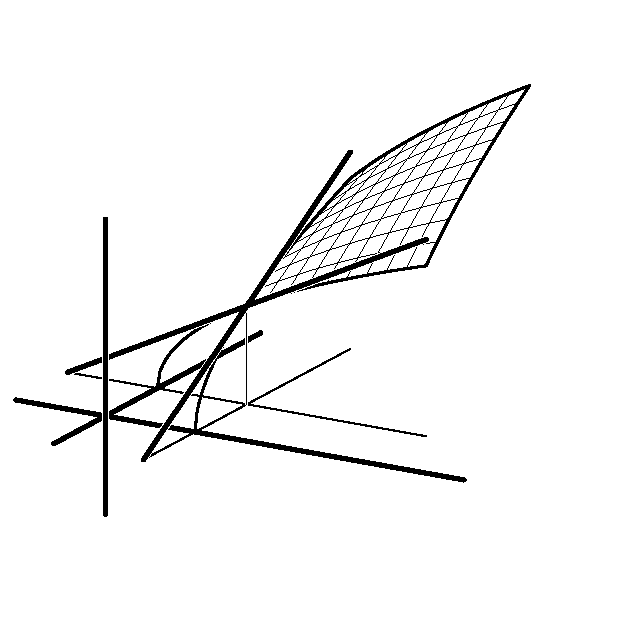
\includegraphics{03two-tangents.pdf}
\end{center}
The tangent plane to the graph (not drawn here, but see
Figure~\ref{fig:total-differential-and-tangent-plane} in the notes)
is the plane containing the two lines in the drawing.
\bigskip

\item[{\bfseries(IV7.8)}]

The function is $f(x, y) = x \ln(xy)$.
We have $f(2, \frac{1}{2}) = 2\ln(2\cdot \frac12) = \ln 1 = 0$.
The gradient of the function is $\nab f = \tvek \ln(xy) + 1  \\
x/y\ttor$.
At the point $(2, \frac{1}{2})$ this is $\nab f = \tvek 1 \\ 4\ttor$,
so the linear approximation is
\[
f(x, y) \approx f(2, \frac{1}{2}) + 1\cdot(x-2)+4\cdot(y-\frac12),
\]
i.e.
\[
f(x, y) \approx 1(x-2) + 4(y-\frac12).
\]
(This is also the answer to problem~\ref{prb:ln-tan-plane}.)

Here we don't want to describe the tangent plan, but we want to find
the value of $f(x, y)$ for $(x,y) = (1.98, 0.4)$.  Substituting these
values of $x$ and $y$ in the linear approximation we get $f(1.98, 0.4)
\approx (1.98-2) + 4 (0.4-0.5) = -0.42$.

This is only an approximation, and you wonder how good it is.  We have
$\Delta x = 1.98-2 = -0.02$, and $\Delta y = 0.4 - \frac12 =
-0.1$\ldots are these numbers ``small''?  To find the error in the
approximation you could use a Lagrange-type remainder term, but that's
not part of math 234.  Instead we grab a calculator and compute
$f(1.98, 0.4) = 1.98\cdot \ln(1.98\cdot 0.4) = -0.46172\cdots$.  So
our linear approximation formula is off by $0.04\cdots$.

\bigskip

\item[{\bfseries(IV7.9a)}]

The $x$-and $y$-axes.
\bigskip

\item[{\bfseries(IV7.9b)}]

The heights are the $z$-coordinates, so $z=xy$ and $z_* = -2+x+2y$.  The
difference is
\[
z-z_* = xy - (-2+x+2y) = xy-x-2y+2.
\]
\bigskip

\item[{\bfseries(IV7.10a)}]
 The tangent plane has equation $z=
ab +b(x-a) + a(y-b) = bx+ay-ab$.
\bigskip

\item[{\bfseries(IV7.10b)}]
 The point $(x, y, z)$ lies on the intersection if $z=xy$ and
$z=bx+ay-ab$.  Therefore $x$ and $y$ must satisfy
$xy-bx-ay+ab = 0$.  This equation factors as follows:
\[
xy-bx-ay+ab = (x-a)(y-b) =0,
\]
so that the intersection contains the line $x=a$, $z=ay$, and
also the line $y=b$, $z=bx$.
\bigskip

\item[{\bfseries(IV10.2)}]

$\pdd{(f+g)}x = f_x + g_x$, and $\pdd{(f+g)}y = f_y + g_y$, so
\[
\vek\pdd{(f+g)}x \\ \rule{0pt}{18pt}\pdd{(f+g)}y \tor
= \vek f_x + g_x \\ f_y + g_y\tor
= \vek f_x \\ f_y\tor + \vek g_x \\g_y\tor
\]
Hence $\nab(f+g) = \nab f + \nab g$.

The product and quotient rules follow in the same way.
\bigskip

\item[{\bfseries(IV10.3b)}]

The gradient is $\nab f = \tvek 2x \\ 8y\ttor$.  This vector is
parallel to $\tvek1\\1\ttor$ if there is a number $s$ such that
$\nab f = s\tvek1\\1\ttor$, i.e.\ $\tvek f_x \\f_y\ttor  = \tvek
s\\s\ttor$.  This happens if $f_x(x, y) = f_y(x, y)$.  From our
computation of the partial derivatives of $f$ we find that $\nab f$ is
parallel to $\tvek1\\1\ttor$ when $2x=8y$.  This happens at every
point on the line $y=\tfrac14x$.

We are asked which points on the level set $f=4$ satisfy this
condition, so we must find where the line $y=\frac14x$ intersects the
level set $x^2 + 4y^2 = 4$.  Solving the two equations gives two
points $(\frac45\sqrt{5}, \frac15\sqrt{5})$ and $(-\frac45\sqrt{5},
-\frac15\sqrt{5})$.

\bigskip

\item[{\bfseries(IV10.3c)}]

$\nab g = \tvek 4y^2 \\ 8xy\ttor$.  This is parallel to
$\tvek1\\1\ttor$ when $y=2x$.  This line intersects the level set
$g=4$ in the point $(\frac12\sqrt[3]{2},\sqrt[3]{2})$.

\textbf{Note: } when you solve the equations $\nab g = \tvek s\\s\ttor$, you
find $y=2x$, but also the line $y=0$ ($x$-axis).
On this line the gradient actually vanishes, i.e.\ $\nab g = \vvv0$
and has no direction, so you can't really say it is parallel to
$\tvek1\\1\ttor$.
\bigskip

\item[{\bfseries(IV10.4a)}]

It's a paraboloid of revolution.
\bigskip

\item[{\bfseries(IV10.4b)}]

$\nab f = \tvek2x\\2y\\-2\ttor = s \tvek1\\1\\2\ttor$ if $-2 = 2s$,
i.e.\ $s=-1$.  This then implies $2x= -1$, $2y = -1$, so that
$x=y=-\frac12$.  Since the point has to lie on the zero set of
$f$, we find $z= \frac12(x^2+y^2) = \frac14$.
\bigskip

\item[{\bfseries(IV10.5a)}]

At $(2,1)$ the gradient is $\nab T = \tvek -2x \\\ -9y^2\ttor =
\tvek-4 \\ -9\ttor$.  To cool off as fast as possible the bug should
go in the opposite direction, i.e.\ in the direction of $\tvek 4 \\
9\ttor$, or any positive multiple of this vector.

\bigskip

\item[{\bfseries(IV10.5b)}]

At $(1,3)$ the gradient is $\nab T = \tvek -2 \\ -81\ttor$.
To keep its temperature constant the bug should walk in any direction
perpendicular to the gradient.  The vector $\tvek 81 \\ -2\ttor$ is
perpendicular to the gradient, so the bug should go in the direction
of $\tvek 81 \\ -2\ttor$ or the opposite direction, $\tvek -81 \\ 2\ttor$.

Any non-zero multiple of $\tvek -81 \\ 2\ttor$ is also a valid answer,
since we can only give the \textit{direction} and not the speed.

Remember: the vector $\tvek -b\\a\ttor$ is perpendicular to
$\tvek a\\b\ttor$.

\bigskip

\item[{\bfseries(IV10.6)}]

The zero set doesn't have to be a curve.  For example the zero set of
the function $f(x, y) = $distance from $(x,y)$ to the square
$Q$ (Problems \ref{prb:distance-to-square-level-sets} and
\ref{prb:distance-to-square-partialderivs}) is the whole square $Q$.
\bigskip

\item[{\bfseries(IV10.7)}]

$\|\nab f\|$ is larger at the top right, because there the
function $f$ changes faster.
\bigskip

\item[{\bfseries(IV10.8a)}]

The gradient at the origin is the zero vector.  This was explained in the text.
\bigskip

\item[{\bfseries(IV10.8b)}]

The function increases in the direction of the gradient.  Since it vanishes on the curve in Figure~\ref{fig:gradientANDlevels}, the function will be positive in the region above the curve, and it will be negative both below the curve and inside the little loop.
\bigskip

\item[{\bfseries(IV10.12b)}]

The result of a rather long calculation is that $\|\nab f\| =1$ everywhere outside the
square, and $\|\nab f\| = 0$ inside the square
(because $f$ is constant in the square.)
\bigskip

\item[{\bfseries(IV10.14)}]

$ax+by+cz = R^2$.
\bigskip

\item[{\bfseries(IV12.1)}]

$4xt\cos(x^2+y^2)+6yt^2\cos(x^2+y^2)$
\bigskip

\item[{\bfseries(IV12.2)}]

$2xy\cos t+2x^2t$
\bigskip

\item[{\bfseries(IV12.3)}]

$2xyt\cos(st)+2x^2s$, $2xys\cos(st)+2x^2t$
\bigskip

\item[{\bfseries(IV12.4)}]

$2xy^2t-4yx^2s$, $2xy^2s+4yx^2t$
\bigskip

\item[{\bfseries(IV12.6a)}]

$\pdd{T_B}{Y} = -\sin\alpha \pdd{T_A}{x} + \cos\alpha \pdd {T_A}{y}$.
\bigskip

\item[{\bfseries(IV12.6b)}]

Take the formulas for $\pdd{T_B}X$ and $\pdd{T_B}Y$ and work out the
right hand side in this problem.
\bigskip

\item[{\bfseries(IV12.9a)}]
 $\vE = -\nab \ln r = \frac{1} {r^2}\tvek x\\ y\ttor$.
\bigskip

\item[{\bfseries(IV12.9b)}]
 $\|\vE\| = 1/r = \frac{1} {\sqrt{x^2+y^2}}$.
\bigskip

\item[{\bfseries(IV12.13a)}]

Height $ = - (x^2-y^2)/(x^2+y^2)$
\bigskip

\item[{\bfseries(IV12.13b)}]

Height $ = \sin 2\theta$.
\bigskip

\item[{\bfseries(IV12.13c)}]

Height $ = \cos 2\varphi$.
\bigskip

\item[{\bfseries(IV15.1)}]
 $f_x=3x^2y^2$, $f_y=2x^3y+5y^4$, $f_{xx}=6xy^2$,
$f_{yy}=2x^3+20y^3$, $f_{xy}=6x^2y$
\bigskip

\item[{\bfseries(IV15.2)}]

$f_x=12x^2+y^2$, $f_y=2xy$, $f_{xx}=24x$, $f_{yy}=2x$, $f_{xy}=2y$
\bigskip

\item[{\bfseries(IV15.3)}]
 $f_x=\sin y$, $f_y=x\cos y$, $f_{xx}=0$, $f_{yy}=-x\sin y$,
$f_{xy}=\cos y$
\bigskip

\item[{\bfseries(IV15.9)}]

A function of two variables has
\[
  f_{xx},\qquad f_{xy}=f_{yx},\qquad f_{yy},
\]
so it has \emph{three} different partial derivatives of second order.

A function of three variables has these partial derivatives:
\[
  \begin{matrix}
    f_{xx} & f_{xy} & f_{xz} \\
    f_{yx} & f_{yy} & f_{yz} \\
    f_{zx} & f_{zy} & f_{zz}
  \end{matrix}
\]
The ones ``below the diagonal'' are the same as corresponding derivatives
above the diagonal, so there are only six different partial derivatives
of second order, namely these:
\[
  \begin{matrix}
    f_{xx} & f_{xy} & f_{xz} \\
    & f_{yy} & f_{yz} \\
    & & f_{zz}
  \end{matrix}
\]
A function of two variables has
\begin{gather*}
  f_{xxx}, \\
  f_{xxy}=f_{xyx}=f_{yxx}, \\
  f_{xyy}=f_{yxy}=f_{yyx},\\
  \text{ and } f_{yyy}
\end{gather*}
so \emph{four} different partial derivatives of third order.
\bigskip

\item[{\bfseries(IV15.15a)}]

We have $g(u,v) = f(u+v, u-v)$, so
\[
  \pdd gu = \pdd fx \pdd{(u+v)}u + \pdd fy \pdd{(u-v)}u
  = f_x(u+v, u-v)+f_y(u+v, u-v).
\]
Similarly,
\[
  \pdd gv = f_x(u+v, u-v) - f_y(u+v, u-v).
\]
Differentiate again to get
\(\DS
  \frac{\pd^2 g}{\pd u^2}
  = f_{xx}(u+v, u-v)+2f_{xy}(u+v, u-v)+f_{yy}(u+v, u-v).
\)
\bigskip

\item[{\bfseries(IV15.15b)}]

\(\DS
\frac{\pd^2 g}{\pd v^2}
= f_{xx}(u+v, u-v)-2f_{xy}(u+v, u-v)+f_{yy}(u+v, u-v)
\)

Note that this is almost the same as $\dfrac{\pd^2g}{\pd u^2}$: the only change is in the minus sign before $f_{xy}$.
\bigskip

\item[{\bfseries(IV15.15c)}]

   $\DS\frac{\pd^2 g}{\pd u\pd v}= f_{xx}(u+v, u-v) - f_{yy}(u+v, u-v)$
\bigskip

\item[{\bfseries(IV15.15d)}]

$\dfrac{\pd^2 g}{\pd u^2} - \dfrac{\pd^2 g}{\pd v^2} = -4f_{xy} $
\bigskip

\item[{\bfseries(IV15.15e)}]

$\dfrac{\pd^2 g}{\pd u^2} + \dfrac{\pd^2 g}{\pd v^2} = 2\bigl(f_{xx}+f_{yy}\bigr)$.
\bigskip

\item[{\bfseries(V3.1a)}]
 If $y\neq0$ then you can increase $x^2-x^3-y^2$ by setting $y=0$.
To put it differently, no matter what you choose for $y$, you always have
\[
  f(x, y) = x^2-x^3-y^2 \leq x^2-x^3  =  f(x, 0).
\]
\bigskip

\item[{\bfseries(V3.1b)}]

The maximum has to appear on the $x$ axis, so the question is
\textit{which $x\geq0$ maximizes $f(x, 0) = x^2-x^3$?}

This is a Math~221 question.  The answer is at $x=2/3$.
\bigskip

\item[{\bfseries(V3.1c)}]

No, $\lim_{x\to-\infty} f(x, y) = +\infty$, so $f$ has no largest value.
\bigskip

\item[{\bfseries(V3.3)}]

\begin{picture} (120.000000,133.111111)(0,0)
    \put(0.0, 0.0){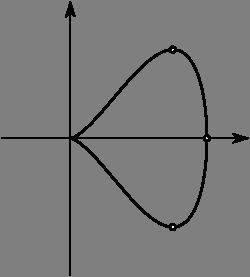
\includegraphics{03onion.pdf}}
        \put(101.33,  68.56){\sffamily\itshape \makebox[0pt][l]{$1$}}
    \put( 82.94, 116.14){\sffamily\itshape \makebox[0pt][c]{$(\frac34, \frac38\sqrt3)$}}
    \put( 82.94,  11.98){\sffamily\itshape \makebox[0pt][c]{$(\frac34, -\frac38\sqrt3)$}}

\end{picture}
%

The quantity $4(x^3-x^4) = 4x^3(1-x)$ is negative when $x<0$ or
$x>1$, so the region is confined to the vertical strip $0\leq x \leq
1$.  Within this strip $R$ is comprised of those points which satisfy
$-\sqrt{4(x^3-x^4)} \leq y \leq +\sqrt{4(x^3-x^4)}$.  The largest
$x$ value is attained at the point with $x=1$, where $y=0$, so, at the
point $(1,0)$.  The smallest $x$ value is attained at the point
$(0,0)$.   The largest $y$ value is attained at the point where
$y^2 = 4x^3-4x^4$ is maximal.  This happens when $x=\frac 34$, and the
largest $y$ value is therefore $\sqrt{4[(3/4)^3-(3/4)^4]} = \frac
38\sqrt{3}$.  The smallest $y$ value also occurs at $x=\frac 34$ and
is given by $y = -\frac 38 \sqrt 3$.
\bigskip

\item[{\bfseries(V6.1a)}]

$f_x = 2x-2$, $f_y = 8y+8$, $f_{xx} = 2$, $f_{xy}=0$, $f_{yy}=8$.

There is exactly one critical point, at $(x, y) = (1,-1)$.

The 2nd order Taylor expansion at this point is
\[
f(1+\Delta x, -1+\Delta y) =
f(1, -1) + (\Delta x)^2 + 4(\Delta y)^2 +\cdots
\]
The quadratic part is positive definite, therefore $f$ has a
\emph{local minimum} at $(1, -1)$.
\bigskip

\item[{\bfseries(V6.1b)}]

$f_x = 2x+6$, $f_y = -2y-10$, $f_{xx} = 2$, $f_{xy}=0$, $f_{yy}=-2$.

There is exactly one critical point, at $(x, y) = (-3,-5)$.

The 2nd order Taylor expansion at this point is
\begin{align*}
  f(-3+\Delta x, -5+\Delta y)
  &= f(-3, -5) + (\Delta x)^2 - (\Delta y)^2 +\cdots \\
  &= f(-3, -5) +\bigl(\Delta x-\Delta y\bigr)\bigl(\Delta x +\Delta
  y\bigr)+\cdots
\end{align*}
The quadratic part factors, therefore $f$ has a
\emph{saddle point} at $(-3, -5)$.  The level set near the critical
point consists of two crossing curves whose tangents are given by the
equations $\Delta x=\Delta y$ and $\Delta x=-\Delta y$.  Since
$\Delta x=x-a=x+3$ and $\Delta y = y-b = y+5$, the two tangent lines
have equations $x+3 = y+5$ and $x+3 = -(y+5)$.
\marginpar{\footnotesize\sffamily
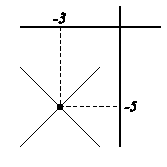
\includegraphics{03answers001.pdf}
\\
Critical point and level set near the critical point.
}%

\bigskip

\item[{\bfseries(V6.1c)}]

$f_x = 2x+4y$, $f_y = 4x+2y$, $f_{xx} = 2$, $f_{xy}=4$, $f_{yy}=2$.
There is one critical point: $(x,y) = (2, -1)$.

The 2nd order Taylor expansion at this point is
\begin{align*}
f(2+\Delta x, -1+\Delta y)
&= f(2, -1) + (\Delta x)^2 + 4 \Delta x \Delta x
            + (\Delta y)^2 +\cdots\\
&= f(2, -1) + \bigl(\Delta x+2\Delta y\bigr)^{2}
            - 3(\Delta y)^2+\cdots\\
&= f(2, -1) + \bigl(\Delta x+(2+\surd3)\Delta y\bigr)
              \bigl(\Delta x+(2-\surd3)\Delta y\bigr)
            +\cdots
\end{align*}
\marginpar{\footnotesize\sffamily
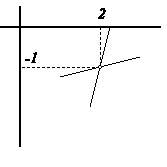
\includegraphics{03answers002.pdf}
\\
Critical point and level set near the critical point.
}%
The quadratic part factors, therefore $f$ has a
\emph{saddle point} at $(2, -1)$.  The level set near the critical
point consists of two crossing curves whose tangents are given by the
equations $\Delta x=-(2+\surd 3)\Delta y$ and $\Delta x=-(2-\surd
3)\Delta y$.  Since $\Delta x=x-a=x-2$ and $\Delta y = y-b = y+1$, the
two tangent lines have equations $x-2 = -(2+\surd3)(y+1)$ and
$x-2 = -(2-\surd3)(y+1)$.
\bigskip

\item[{\bfseries(V6.1d)}]

$f_x = 2x-y-5$, $f_y = -x+4y+6$, $f_{xx} = 2$, $f_{xy}=-1$, $f_{yy}=4$.

There is again one critical point: $x=2$, $y=-1$.

The 2nd order Taylor expansion at this point is
\begin{align*}
f(2+\Delta x, -1+\Delta y)
&= f(2, -1) + (\Delta x)^2 - \Delta x \Delta x
            + 2(\Delta y)^2 +\cdots\\
&= f(2, -1) + \bigl(\Delta x-\tfrac12\Delta y\bigr)^{2}
            +\tfrac74(\Delta y)^2+\cdots
\end{align*}
The second order part of the Taylor expansion is positive, so
$(2, -1)$ is a \emph{local minimum}.

\bigskip

\item[{\bfseries(V6.1e)}]

$f_x = -36x+4x^3$, $f_y = 2y$, $f_{xx} = -36+12x^2$, $f_{xy}=0$,
$f_{yy}=2$.

The equation $f_x=0$ has three solutions, $x=0$ and $x=\pm3$.
The equation $f_y=0$ has only one solution $y=0$.
Therefore there are three critical points, the origin and the points
$(\pm 3,0)$.

The taylor expansions at these points are
\begin{align*}
    f(\Delta x, \Delta y)
    &= f(0,0) -18 (\Delta x)^2 + (\Delta y)^2 + \cdots \\
    &= f(0,0) + \bigl(\Delta y-\sqrt{18} x\bigr)\bigl(\Delta y+\sqrt{18} x\bigr)
              + \cdots \\
    f(3+\Delta x, \Delta y)
    &= f(3,0) +36 (\Delta x)^2 + (\Delta y)^2 + \cdots \\
    f(-3+\Delta x, \Delta y)
    &= f(-3,0) +36 (\Delta x)^2 + (\Delta y)^2 + \cdots
\end{align*}
The second order terms in the Taylor expansions at $(3,0)$ and at
$(-3,0)$ are both positive for all $\Delta x$ and $\Delta y$, so both
points $(\pm3, 0)$ are local minima.  The second order part of the
expansion at the origin factors and hence the origin is a saddle
point.  The tangents to the zeroset at the origin are the lines
$\Delta y = \pm \sqrt{18}\Delta x = \pm 3\sqrt2 \Delta x$.  Since here
$\Delta x = \text{``}x-a\text{''} = x$, and $\Delta y = y$, the
tangents are the lines through the origin given by $y=\pm 3\sqrt2 x$.

You can try to draw the zeroset of this function and analyze it in the
same way as the ``fishy example'' in \ref{sec:critical-fish}.  The
zeroset of $f$ consists of the graphs of $y = \pm \sqrt{18x^2-x^4} =
\pm |x|\sqrt{18-x^2}$.
It looks like a squashed ``$\infty$'' or a butterfly (you decide.)
\marginpar{\footnotesize\sffamily
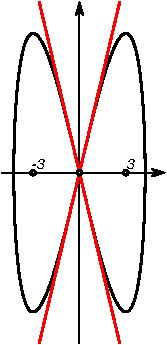
\includegraphics{03answers003.pdf}
\\
Critical points and zero set.
}
\bigskip

\item[{\bfseries(V6.1f)}]

There are nine critical points. Four global minima at $(\pm 3,
\pm\sqrt{3})$, four saddle points at $(0,\pm\sqrt{3})$ and $(\pm3,0)$
respectively, and finally, a local but not global maximum at the
origin.
\bigskip

\item[{\bfseries(V6.1g)}]
 critical point at $(1,-1/6)$
$f_x = 4-4x$, $f_y = -1-6y$, $f_{xx} = -4$, $f_{xy}=0$, $f_{yy}=-6$.

Second order Taylor expansion at the critical point:
\[
f(-1+\Delta x, -\tfrac16+\Delta y) = f(1, -\tfrac16)
-2(\Delta x)^2-3(\Delta y)^2 + \cdots
\]
The second order terms are always negative so $(1, -\tfrac16)$ is a
local maximum.
\bigskip

\item[{\bfseries(V6.1h)}]
 The derivatives are:
\[
f_x = 4y-2xy-2y^2,\quad f_y = 4x-x^2-4xy,\quad f_{xx} = -2y,\quad
f_{xy}=4-2x-4y,\quad f_{yy}=-4x.
\]
This function is given in factored form, so without solving the
equations $f_x=0$, $f_y=0$ you can say the following about this
problem.  The zero set consists of the three lines: the $y$-axis
($x=0$), the $x$-axis ($y=0$) and the line with equation $4-x-2y=0$.
It follows that the intersection points $(0,0)$, $(4,0)$, and $(0,2)$
of these lines are saddle points.  Since $f>0$ in the triangle formed
by the three lines this triangle must contain at least one local
maximum.

\begin{center}
  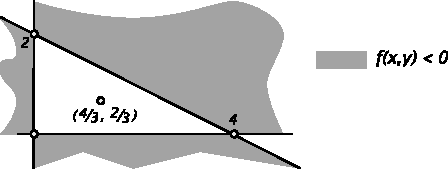
\includegraphics{03answers004.pdf}
\end{center}
To find all critical points solve these equations:
\[
f_x = 4y-2xy-2y^2 = 0 \iff \text{\framebox{$y=0$ or $4-2x-2y=0$}}
\]
and
\[
f_y = 4x-x^2-4xy=0  \iff \text{\framebox{$x=0$ or $4-x-4y=0$}}
\]
Since both equations $f_x=0$ and $f_y=0$ lead to two possibilities, we
have to consider $2\times 2=4$ cases:
\begin{description}
  \item[$y=0$ \& $x=0$] This tells us the origin is a critical point
  \item[$y=0$ \& $4-x-4y=0$] Solving these equations leads to
    $x=4, y=0$, so $(4,0)$ is a critical point.
  \item[$4-2x-2y=0$ \& $x=0$] Solve and you find that $(0,2)$ is a
    critical point.
  \item[$4-2x-2y=0$ \& $4-x-4y=0$] Solve these equations and you get
    $(x,y) = (\tfrac43, \tfrac23)$.
\end{description}
The first three critical points are the saddle points we predicted.
The fourth critical point must be a local maximum, since there has to
be one in the triangle, and of all the critical points we have found
the others are all saddle points.
\bigskip

\item[{\bfseries(V6.1i)}]

Two saddle points:  $(0,0)$ and $(1,1)$.
\bigskip

\item[{\bfseries(V6.1j)}]
 Two saddle points:  $(2,2)$ and $(-2,-2)$
%$f_x = <++>$, $f_y = <++>$, $f_{xx} = <++>$, $f_{xy}=<++>$, $f_{yy}=<++>$.
\bigskip

\item[{\bfseries(V6.1l)}]
 The origin. Neither a local max, min, nor saddle.
The graph of this function is called the ``Monkey Saddle'' as
it accommodates two legs and a tail too.  Draw it in your graphing
program to see this.
\bigskip

\item[{\bfseries(V6.1m)}]

Zero set is the parabola with equation $x=y^2$, and the line
$x=1$.  They intersect at $(1, \pm1)$, so the function has two saddle
points $(1,1)$ and $(1,-1)$.  The region between the line $x=1$ and
the parabola must contain  local minimum.  It is located at
$(\frac12, 0)$.
\bigskip

\item[{\bfseries(V6.1n)}]
 Two saddle points : $(2,2)$ and $(-2,-2)$.
Yes, this problem appeared twice.
\bigskip

\item[{\bfseries(V6.1o)}]
  All points on the $y$-axis are critical points.  They are all
global minima, but the second derivative test doesn't tell you so.
\bigskip

\item[{\bfseries(V6.1p)}]

All points on the $y$-axis are again critical points.  Those with
$y>0$ are local minima, those with $y<0$ are local maxima, and the
origin is neither.  The second derivative test applies to none of
these points.
\bigskip

\item[{\bfseries(V6.1q)}]
  All points on the unit circle are global minima, because the
function vanishes there, and is positive everywhere else.  The origin
is a local maximum.  The 2nd derivative test applies to the origin,
but not to any of the other critical points.
\bigskip

\item[{\bfseries(V6.1r)}]

All points on the $y$-axis are again critical points.  Those with
$y>0$ are local minima, those with $y<0$ are local maxima, and the
origin is neither.  The second derivative test applies to none of
these points.
\bigskip

\item[{\bfseries(V6.5a)}]
  $(3,4/3)$
\bigskip

\item[{\bfseries(V6.5c)}]

$x= (a+c+e)/3$, $y=(b+d+f)/3$.
\bigskip

\item[{\bfseries(V6.6)}]

You have to show that $f_x(a, b) = f_y(a, b) = 0$.
By the product rule $f_x(a, b) = g_x(a, b)h(a, b) + g(a, b) h_x(a,
b)$.  Since both $g(a, b) = 0$ and $h(a, b) = 0$, it follows that
$f_x(a, b) = 0$.   The same reasoning applies to $f_y(a, b)$.
\bigskip

\item[{\bfseries(V8.1a)}]

One variable calculus!  There is only one variable, $a$, and we must
solve $E'(a) = 0$.
\bigskip

\item[{\bfseries(V8.1b)}]

$a= (x_1+\cdots+x_N)/N$, i.e.\ the average provides ``the best fit.''
\bigskip

\item[{\bfseries(V8.2a)}]
 Three:  $a$, $b$, and $c$.
\bigskip

\item[{\bfseries(V8.2b)}]
 The equations for $(a, b, c)$ are:
\[
\begin{array}{rlcrlcrlrcl}
    (\tsum x_k^4)&a &+&(\tsum x_k^3)&b &+& (\tsum x_k^2)&c
    &=& \tsum x_k^2y_k\\[1ex]
    (\tsum x_k^3)&a &+&(\tsum x_k^2)&b &+& (\tsum x_k)&c
    &=& \tsum x_ky_k\\[1ex]
    (\tsum x_k^2)&a &+&(\tsum x_k)&b &+& N&c &=& \tsum y_k
\end{array}
\]
\bigskip

\item[{\bfseries(V8.3)}]
 The equations are
\[
\begin{array}{rlcrlcrlrcl}
    (\tsum x_k^2)&a &+&(\tsum x_ky_k)&b &+& (\tsum x_k)&c
    &=& \tsum x_kz_k\\[1ex]
    (\tsum x_ky_k)&a &+&(\tsum y_k^2)&b &+& (\tsum y_k)&c
    &=& \tsum y_kz_k\\[1ex]
    (\tsum x_k)&a &+&(\tsum y_k)&b &+& N&c &=& \tsum z_k
\end{array}
\]
\bigskip

\item[{\bfseries(V10.1)}]

The two $\Delta x$ and $\Delta y$'s are different.  The first set of $(\Delta
x,\Delta y)$ are
\[
  \Delta x = x-0, \qquad \Delta y = y-0,
\]
$(0,0)$ being the coordinates of the first critical point we studied.  The second set
of $(\Delta x,\Delta y)$ is
\[
  \Delta x = x-\tfrac23, \qquad \Delta y = y-0,
\]
where $(\frac23, 0)$ is the other critical point.  In a drawing:
\begin{figure}[h]
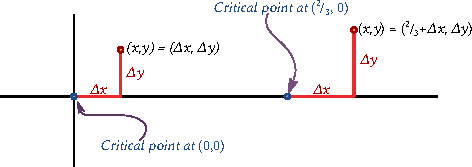
\includegraphics{answer-whichDxDy.pdf}
\end{figure}
\bigskip

\item[{\bfseries(V10.2a)}]

$f(\Delta x, \Delta y)
= \Bigl(1-\Delta x+\Delta x\Delta y\Bigr)^2
= 1-2\Delta x+\Delta x^2+2\Delta x\Delta
y+\cdots$
\bigskip

\item[{\bfseries(V10.2b)}]

$f(1+\Delta x, 1+\Delta y)
= \Bigl(1-(1+\Delta x)+(1+\Delta x)(1+\Delta y)\Bigr)^2
=
1+2\Delta y+2\Delta x\Delta y+2(\Delta y)^2+\cdots$
\bigskip

\item[{\bfseries(V10.2c)}]

$f(\Delta x,\Delta y) = e^{\Delta x-(\Delta y)^2} =
1+\Delta x+\frac{1}{2}(\Delta x)^2 -(\Delta y)^2+\cdots$
\bigskip

\item[{\bfseries(V10.2d)}]

$f(1+\Delta x, 1+\Delta y)
= e^{(1+\Delta x)-(1+\Delta y)^2}
=
1+\Delta x - 2\Delta y+ \frac{1}{2}(\Delta x)^2 - 2\Delta x\Delta y
+(\Delta y)^2+\cdots$
\bigskip

\item[{\bfseries(V10.4)}]
  Complete the square and you get
\[
Q(x, y) = \bigl(x-ay\bigr)^2 + \bigl(1- a^2\bigr)y^2.
\]
When $1-a^2>0$, i.e.\ when $-1<a<1$ the form is positive definite.
When $a=\pm 1$ the form is a perfect square, namely,
\[
x^2 \pm 2xy + y^2 = \bigl(x\pm y\bigr)^2.
\]
When $1-a^2<0$, i.e.\ when $a>1$ or $a<-1$, the form is indefinite:
\[
x^2 + 2axy + y^2 =
\Bigl(x-ay-\sqrt{a^2-1}y\Bigr)
\Bigl(x-ay+\sqrt{a^2-1}y\Bigr)
=(x-k_+y)(x-k_-y),
\]
where $k_\pm = -a \pm \sqrt{a^2-1}$.

\bigskip

\item[{\bfseries(V10.5)}]

See the solutions to Problem \ref{prb:find-critical-points} for the
solutions to this problem.
\bigskip

\item[{\bfseries(V10.7a)}]

$f_x = 2x-\frac12y^2$, $f_y = 2y-xy$.
The equation $f_y=y(2-x)=0$ leads to two possibilities: $x=2$ or
$y=0$.  If $y=0$ then $f_x=0$ implies $x=0$, which gives us one
critical point, the origin $(0,0)$.  If on the other hand $x=2$, then
$f_x=0$ implies $y^2=8 \iff y=\pm2\sqrt{2}$.  We therefore get two
more critical points $(2, \pm 2\sqrt{2})$.

The second derivatives are $f_{xx} = 2$, $f_{xy} = -y$, $f_{yy} =
2-x$.  Therefore we have the following Taylor expansions at the
three critical points:
\begin{align*}
    f(\Delta x, \Delta y)
    &= f(0,0) + (\Delta x)^2 + (\Delta y)^2 + \cdots
    &\implies \text{loc.min.}\\
    f(2+\Delta x, 2\sqrt{2} + \Delta y)
    &= f(2, 2\sqrt{2}) + (\Delta x)^2 - 2\sqrt{2} \Delta x \Delta y +
    0(\Delta y)^2+\cdots\\
    &= f(2, 2\sqrt{2}) + \bigl(\Delta x - 2\sqrt{2} \Delta y\bigr)
    \Delta x +\cdots
    &\implies \text{saddle}\\
    f(2+\Delta x, -2\sqrt{2} + \Delta y)
    &= f(2, -2\sqrt{2}) + (\Delta x)^2 + 2\sqrt{2} \Delta x \Delta y +
    0(\Delta y)^2+\cdots\\
    &= f(2, -2\sqrt{2}) + \bigl(\Delta x + 2\sqrt{2} \Delta y\bigr)
    \Delta x +\cdots
    &\implies \text{saddle}
\end{align*}
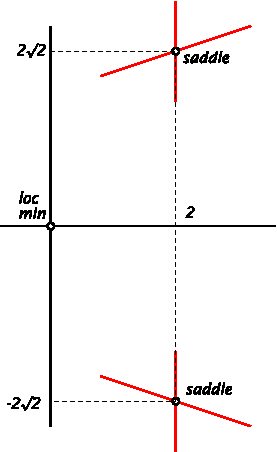
\includegraphics[width=96pt]{03answers005.pdf}
The origin is therefore a local minimum, and the points $(2,
\pm2\sqrt{2})$ are saddle points.  At $(0, 2\sqrt{2})$ the level set
consists of two crossing curves, whose tangents are given by
$\Delta x=0$ (a vertical line) and $\Delta x=2\sqrt{2}\Delta y$ (a line
with slope $1/2\sqrt{2} = \frac14\sqrt{2}$).
\bigskip

\item[{\bfseries(V10.7c)}]

$f_x = 1-y^2$, $f_y = 2-2xy$.
Critical points: $f_x=0$ holds when $y=\pm 1$.  If $y=+1$, then
$f_y=0$ implies $x=1$, and if $y=-1$ then $f_y=0$ implies $x=-1$.
There are therefore two critical points, $(1,1)$ and $(-1,-1)$.
\bigskip

\item[{\bfseries(V13.1)}]

$f(x, y) = xy$, $g(x, y) = x^2 + \frac14 y^2$.
$\nab f = \tvek y \\ x\ttor$, $\nab g = \tvek 2x\\ y/2\ttor$.

First we check for possible max/minima which satisfy $\nab g=\vvv0$.
But the only point $(x,y)$ satisfying $\nab g(x,y) = \tvek0\\0\ttor$
is the origin $(x, y) = (0,0)$, and this point does not lie on the
constraint set.

Therefore, \textbf{if} there is a minimum it is attained at a solution
of Lagrange's equations
\begin{align*}
  f_x = \lambda g_x &\iff y = 2\lambda x \\
  f_y = \lambda g_y &\iff x = \lambda y/2 \\
  g(x, y) = 1 & \iff x^2+\tfrac14 y^2 = 1
\end{align*}
Multiply the first equation with $y$ and the second with $4x$, then
you get
\[
y^2 = 2\lambda xy \text{ and } 4x^2 = 2\lambda xy
\]
Hence $y^2 = 4x^2$.  Put that in the constraint, and you find
\[
1=x^2 + \tfrac14 y^2 = 2 x^2.
\]
Thus $x= \pm\sqrt{1/2} = \pm \frac12 \sqrt{2}$ and $y = \pm \sqrt2$.
In all we have found \emph{four} possible solutions.
Lagrange's method does not tell us which, if any, of these are minima.
\marginpar{\footnotesize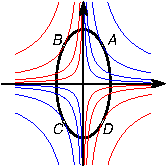
\includegraphics{03answers006.pdf}\\
Level sets of the function $f(x, y) = xy$ and the constraint set
$x^2+\frac14y^2=1$}

By looking at the constraint set (it's an ellipse with horizontal axis
of length 1 and vertical axis of length 2) and taking into account
that $f(x, y) =xy$ is positive in the first and third quadrants, and
negative in the second and fourth, you find out that the two points
$(\frac12\sqrt{2},\sqrt{2})$ and $(-\frac12\sqrt{2},-\sqrt{2})$  ($A$
and $C$ in the figure) are maximum points, while
$(-\frac12\sqrt{2},\sqrt{2})$ and $(\frac12\sqrt{2},-\sqrt{2})$  ($B$
and $D$ in the figure) are minimum points.
\bigskip

\item[{\bfseries(V13.2a)}]

Let the sides of the box be $x,y,z$.  We want to minimize the quantity $A =
2xy+2yz+2xz$, with the constraint $V=xyz=\frac12$.  The constraint implies that
$x\neq0$, $y\neq0$ and $z\neq0$ moreover, given $x$ and $y$ the only $z$
which satisfies the constraint is $z=1/(2xy)$.  Thus we must minimize the
following function of two variables
\[
A(x,y) = xy + \frac{1} {2x} + \frac{1} {2y}
\]
over all $x>0$, $y>0$.

A minimum must be an interior minimum (can't be on the $x$ or $y$-axis
since these are excluded), and thus must be a critical point.
\[
\pdd Ax = y-\frac{1} {2x^2}, \qquad
\pdd Ay = x - \frac{1} {2y^2}.
\]
Solving $A_x=A_y=0$ for $(x,y)$ leads to $x=y=\sqrt[3]2$, so the solution
is a cube $1/\sqrt[3]{2}$ on a side
\bigskip

\item[{\bfseries(V13.2b)}]

We wish to minimize $A(x,y,z) = 2yz+2xz+2xy$ with constraint
$V(x, y, z) = xyz = \frac12$, using Lagrange's method.

First we check for exceptional points on the constraint set, i.e.\
points $(x,y,z)$ that satisfy both $V(x, y, z) = \frac12 $ and
$\nab V(x, y, z) = \vvv0$.  Since
\[
\nab V = \vek yz \\ xz\\ xy\tor
\]
the gradient $\nab V$ vanishes if at least two of the three
coordinates $x, y, z$ are zero.  But such a point can never satisfy
the constraint $xyz=\tfrac12$.  Therefore, if there is a box with
least area, its sides $x, y, z$ must satisfy Lagrange's equations.

Lagrange's equations are
\begin{align*}
  A_x = \lambda V_x &\iff 2y+2z = \lambda yz\\
  A_y = \lambda V_y &\iff 2x+2z = \lambda xz\\
  A_z = \lambda V_z &\iff 2x+2y = \lambda xy
\end{align*}
To get rid of $\lambda$ multiply the first equation with $x$ and the
second with $y$ to get
\[
y(2x+2z) = \lambda xyz = x(2y+2z) \implies
2xy+2yz = 2xy+2xz \implies 2yz=2xz.
\]
Therefore we find that either $z=0$ or $x=y$.
But $z=0$ is not possible, because $(x,y,z)$ must satisfy the
constraint $xyz=0$.  Therefore we get $x=y$.

If you multiply the second Lagrange equation with $y$ and the third
with $z$ then the same reasoning as above tells you that $y=z$.

So, \emph{if there is a minimum} then it happens when $x=y=z$, i.e.\
when the box is a cube.  The only cube that satisfies the constraint
has sides $x=y=z=2^{-1/3}$.

As always, Lagrange's method does not rule out the possibility that
the cube we have found actually maximizes the surface area, rather
than minimizing it.  That this is actually not the case is something
you would have to prove by other means.  We will not do that in this
course.

\bigskip

\item[{\bfseries(V13.3)}]
  Answer: the shortest distance is $\sqrt{100/3}$.

Solution:  If $(x, y, z)$ is any point than its distance to the origin
is $d(x, y, z) = \sqrt{x^2+y^2+z^2}$.  We want to minimize $d(x, y,
z)$ over all points $(x, y, z)$ which satisfy the constraint
$g(x, y, z) = x+y+z=10$.  Instead of minimizing $d(x, y, z)$ we will
minimize $f(x, y, z) = d(x, y, z)^2 = x^2+y^2+z^2$.  You can do this
problem directly with the function $d(x,y,z)$ and you will get the
same answer -- the computations are just a little longer because
$f$ has easier derivatives than $d$.

We use Lagrange's method.  First we check for exceptional points,
i.e.\ points on the constraint set which satisfy $\nab g=\vvv0$.
Since $\nab g = \tvek1\\1\\1\ttor$ the gradient of $g$ can never be
the zero vector, so there are no exceptional points.  If there is a
minimum of $f$ on the constraint set, it must be a solution of
Lagrange's equations.

The Lagrange equations are
\begin{align*}
  f_x=\lambda g_x &\iff 2x = \lambda\\
  f_y=\lambda g_y &\iff 2y=\lambda\\
  f_z=\lambda g_z &\iff 2z=\lambda
\end{align*}
Therefore \emph{if there is a nearest point to the origin on the
plane} then it must satisfy $x=y=z=\lambda/2$ as well as the
constraint.  The only point satisfying these conditions is
$(\tfrac{10}3,\tfrac{10}3,\tfrac{10}3)$.

Lagrange's method does not tell us that this is the nearest point. As
far as Lagrange is concerned it could also be the furthest point from
the origin.  (But because we know what a plane looks like we ``know''
that there has to be a nearest point to the origin.)


\bigskip

\item[{\bfseries(V13.5a)}]

Minimize $f(x, y, z) = (x-2)^2 + (y-1)^2 + (z-4)^2$ subject to the
constraint $g(x, y, z) = 2x-y+3z = 1$.

First, since $\nab g - \tvek 2 \\ -1 \\ 3\ttor \neq \vvv0$, there are
no exceptional points, so the nearest point (if it exists) is a
solution of Lagrange's equations.  These are
\[
2(x-2) = 2\lambda, \quad
2(y-1) = -\lambda, \quad
2(z-4) = 3\lambda.
\]
Eliminate $\lambda$ to get
\[
x=-2y+4, \qquad
z = -3y+7.
\]
Combined with the constraint you then find
\[
y= 2,\quad x=  0, \quad z= 1.
\]
The Lagrange multiplier is $\lambda = x-2 = -2$.

The distance from the point we found to the given point $(2, 1, 4)$ is
\[
d = \sqrt{(x-2)^2 + (y-1)^2 + (z-4)^2}
=\sqrt{14}
\]
\bigskip

\item[{\bfseries(V13.5b)}]

$|ax_0+by_0+cz_0-d|/\sqrt{a^2+b^2+c^2}$
\bigskip

\item[{\bfseries(V13.8)}]
  a cube
\bigskip

\item[{\bfseries(V13.10)}]
  $65/3\times 65/3\times 130/3$
\bigskip

\item[{\bfseries(V13.11)}]
  It has a square base, and is one and one half times as tall
as wide.  If the volume is $V$ the dimensions are $\root 3 \of {2V/3}\times
\root 3 \of {2V/3}\times \root 3\of {9V/4}$.
\bigskip

\item[{\bfseries(V13.12)}]
  $(0,0,1)$, $(0,0,-1)$
\bigskip

\item[{\bfseries(V13.13)}]
  $\root 3\of{4V}\times\root
3\of{4V}\times\root 3\of{V/16}$
\bigskip

\item[{\bfseries(V13.14)}]
  Farthest: $(-\sqrt2,\sqrt2,2+2\sqrt2)$; closest:
$(2,0,0)$, $(0,-2,0)$
\bigskip

\item[{\bfseries(VI3.1a)}]
 %%%%%%%%%%%%%%%%%%%%%%%%%%%%%%%%%%%%%%%%%%%%%%%%%
$2$
\bigskip

\item[{\bfseries(VI3.1b)}]
 %%%%%%%%%%%%%%%%%%%%%%%%%%%%%%%%%%%%%%%%%%%%%%%%%
$8$
\bigskip

\item[{\bfseries(VI3.1c)}]

$2/3$
\bigskip

\item[{\bfseries(VI3.1d)}]

$\DS \int_0^\pi \int _0^y \frac{\sin y}{y}\; dx\; dy
=
\int_0^\pi \frac{\sin y}{y} \cdot y \; dy = \int_0^\pi \sin y \; dy =
2$.
\bigskip

\item[{\bfseries(VI3.1e)}]

Except for a change in notation ($y\to\theta$ and $x\to r$) this is
the same integral as in the previous problem.  The answer is again $2$.
\bigskip

\item[{\bfseries(VI3.1f)}]

Which function is being integrated?  It's the function $f(x, y) = 1$.

\noindent
$\int_0^1 \int _0^{\sqrt{1-x^2}}\; dy\; dx
=\int_0^1 \bigl[y\bigr]_{y=0}^{y=\sqrt{1-x^2}}\; dx
= \int_0^1 \sqrt{1-x^2}\; dx$.
The last integral
is the area of a quarter circle with radius 1, so the answer is $\pi/4$.
\bigskip

\item[{\bfseries(VI3.2)}]

Once you compute the inner integral
\[
\int_0^1 \sin(\pi x) dx  = \left[ -\frac1\pi\cos\pi x \right]_{x=0}^1
=-\frac1\pi\cos \pi - \frac1\pi/4 (-\cos 0) = 2,
\]
you get
\[
\int_x^1 \Bigl\{\int_0^1 \sin(\pi x) dx \Bigr\}dy
=\int_x^1 2dy = \left[ 2y \right]_{y=x}^1 = 2(1-x).
\]
The result depends on $x$.  The $x$ in the answer and the two $x$-es
in the inner integral refer to different quantities.  This is at best
confusing, and should really never be done.
\bigskip

\item[{\bfseries(VI3.3a)}]

Not true!
To give a counterexample for the statement in the problem, almost any
two functions $f$ and $g$ will do.  For instance, if you choose $f(x) = x$, $g(y)=1$, then you get
\[
\int_0^1 \int_0^2 f(x) g(y) \; dx\; dy= \int_0^1\int_0^2 xdx dy = 2.
\]
but
\[
\int_0^1 f(x) \; dx\; \times\;
\int_0^2 g(y)\; dy
=
\int_0^1 x \; dx\; \times\;
\int_0^2  dy
=
\frac{1}{2}\times2 = 1.
\]
\bigskip

\item[{\bfseries(VI3.3b)}]

True!
\[
  \int_0^1\int_0^2 f(x)g(y) dy dx
  =\int_0^1\left\{ \int_0^2 f(x)g(y) dy \right\}dx .
\]
Since $f(x)$ does not depend on $y$, we have
\[
\int_0^2 f(x)g(y) dy=f(x) \int_0^2 g(y)\, dy.
\]
Therefore
\[
  \int_0^1\left\{ \int_0^2 f(x)g(y) dy \right\}dx
  =\int_0^1 f(x) \left\{\int_0^2 g(y) dy \right\}dx .
\]
The integral $\int_0^2 g(y)dy$ is a constant, and does therefore not depend on $x$,
so we can factor it out of the $x$-integral:
\[
  \int_0^1 f(x) \left\{\int_0^2 g(y) dy \right\}dx
  = \int_0^1 f(x)\, dx \cdot \int_0^2 g(y)\, dy,
\]
which is what we had to show.
\bigskip

\item[{\bfseries(VI3.3c)}]

This is false, and there is no simple way of fixing it.  To see that this fails
evaluate both sides with $f(x) = 1$ and $g(y)$.  On the left you get the area of
the disc $D$, which is $\pi$, and on the right you get $2\cdot2=4$.
\bigskip

\item[{\bfseries(VI3.4)}]

The volume under the graph is
$\frac13 ba^3 + \frac13 ab^3 = \frac 13 ab(a^2+b^2)$.
The volume of the surrounding block is $a\times b\times (a^2+b^2)$, so
the region beneath the graph occupies one third of the surrounding
block, no matter which $a$ or $b$ you choose.
\bigskip

\item[{\bfseries(VI3.5a)}]

$16$
\bigskip

\item[{\bfseries(VI3.5b)}]

$4$
\bigskip

\item[{\bfseries(VI3.5c)}]

$15/8$
\bigskip

\item[{\bfseries(VI3.5d)}]

$1/2$
\bigskip

\item[{\bfseries(VI3.5e)}]

$5/6$
\bigskip

\item[{\bfseries(VI3.5f)}]

$12-65/(2e)$.
\bigskip

\item[{\bfseries(VI3.5g)}]

$1/2$
\bigskip

\item[{\bfseries(VI3.5h)}]

$(2/9)2^{3/2}-(2/9)$
\bigskip

\item[{\bfseries(VI3.5i)}]

$(1-\cos(1))/4$
\bigskip

\item[{\bfseries(VI3.5j)}]

$(2\sqrt2-1)/6$
\bigskip

\item[{\bfseries(VI3.5k)}]

$\pi-2$
\bigskip

\item[{\bfseries(VI3.6a)}]

$8\pi$
\bigskip

\item[{\bfseries(VI3.6b)}]

$2$
\bigskip

\item[{\bfseries(VI3.6c)}]

$5/3$
\bigskip

\item[{\bfseries(VI3.6d)}]

$81/2$
\bigskip

\item[{\bfseries(VI3.6e)}]

$2a^3/3$
\bigskip

\item[{\bfseries(VI3.6f)}]

$8\pi$
\bigskip

\item[{\bfseries(VI3.6g)}]

$\pi/32$
\bigskip

\item[{\bfseries(VI3.8a)}]

$A$
\bigskip

\item[{\bfseries(VI3.8b)}]

$B/2$
\bigskip

\item[{\bfseries(VI3.9a)}]

$\DS\int_0^1 \int_0^{\sqrt{1-x^2}} \frac{2xy}{x^2+y^2}\; dy\; dx$.
\bigskip

\item[{\bfseries(VI3.9b)}]

In P.C.\ the function simplifies to $F(r,\theta) = 2\sin \theta\cos
\theta$, so the volume is
\[
V = \int_0^1 \int_0^{\pi/2} 2\sin\theta\cos\theta r\; d\theta\; dr
=\int_0^1 \left[ \sin^2\theta \right]_0^{\pi/2} r\; dr
=\tfrac12.
\]
\bigskip

\item[{\bfseries(VI7.1a)}]

A cone around the positive $z$ axis, with opening angle $\pi/6.$
\bigskip

\item[{\bfseries(VI7.1b)}]

The negative half of the $z$ axis.
\bigskip

\item[{\bfseries(VI7.1c)}]

The $xy$ plane.
\bigskip

\item[{\bfseries(VI7.1d)}]

The half of the $yz$ plane which contains the positive $y$ axis, and
which ends at the $z$-axis.
\bigskip

\item[{\bfseries(VI7.2a)}]

$0\leq \theta\le\pi/2$, $0\le \rho\le a$, $0\le\phi\le\pi/2$.
\bigskip

\item[{\bfseries(VI7.2b)}]

$0\le\theta\le\pi/2$, $0\le r\le a$, $0\le z\le \sqrt{a^2-r^2}$, or:

$0\le\theta\le\pi/2$, $0\le z\le a$, $0\le r\le \sqrt{a^2-z^2}$.
\bigskip

\item[{\bfseries(VI7.3)}]

Figures \ref{fig:04cylindrical-volume-element} and
\ref{fig:04spherical-volume-element}.
\bigskip

\item[{\bfseries(VI7.4a)}]

Large circle has radius $1$, the smaller has radius $\sqrt{1-z^2}$.
\bigskip

\item[{\bfseries(VI7.4b)}]

$x=\sqrt{1-y^2-z^2}$ for the point in front, and $x=-\sqrt{1-y^2-z^2}$
for the point in the back (furthest away from you, the viewer).
\bigskip

\item[{\bfseries(VI7.5a)}]

The potential energy is ``mass$\times$height$\times g$''.  The mass of
the small piece of honey is $\Delta m = \mu\times \Delta V$, where
$\Delta V$ is the volume occupied by the small piece of honey.  This
is not an exact formula, but only an approximation, since not all
particles in the small piece of honey have exactly the same height.
However, as one considers smaller and smaller pieces the approximation
gets better.
\bigskip

\item[{\bfseries(VI7.5b)}]

The total potential energy is
\[
\text{P.E.} = \liiint _D \mu g z \; dV.
\]
Interpretation: this is the total energy that would be released if you
put all the honey at height zero (e.g.\ by pouring it out of the jar
onto the floor.)
\bigskip

\item[{\bfseries(VI7.5c)}]

The iterated integral is
\[
\text{P.E.} =
\int_{x=0}^A \int_{y=0}^B \int_{z=0}^{f(x, z)} \mu g z \; dz\; dy\;
dx
=
\frac12 \mu g
\int_{x=0}^A \int_{y=0}^B f(x, y)^2 \; dy\; dx.
\]
\bigskip

\item[{\bfseries(VI7.6a)}]

The kinetic energy in a small region of the airmass is $\frac12 \Delta
m \times v^2$, where $\Delta m$ is the mass of the air in the small
region.  This mass is $\mu\times \Delta V$, with $\Delta V$ the
volume of the small region, so the kinetic energy of the small region
is $\frac 12 \mu \times v^2\times\Delta V$.  Partitioning the
whole airmass, and adding the kinetic energies of all the small pieces
leads to this integral:
\[
\text{K.E.} = \liiint_D \tfrac12\mu v(r)^2\; dV
= \tfrac12\mu \liiint_D v(r)^2\; dV
.\]
\bigskip

\item[{\bfseries(VI7.6b)}]

In cylindrical coordinates the domain is defined by $0\le r\le R$ and
$0< z \le H$, so the integral is
\[
\text{K.E.}
=
\frac 12
\int_{\theta=0}^{2\pi}\int_{z=0}^{H}\int_{r=0}^R
\frac{r}{1+r^2}\; dr\; dz\; d\theta
=
\frac{\pi}{2}H\ln\bigl(1+R^2\bigr).
\]
\bigskip

\item[{\bfseries(VI7.7a)}]

$623/60$
\bigskip

\item[{\bfseries(VI7.7b)}]

$-3e^2/4+2e-3/4$
\bigskip

\item[{\bfseries(VI7.7c)}]

$1/20$
\bigskip

\item[{\bfseries(VI7.7d)}]

$\pi/48$
\bigskip

\item[{\bfseries(VI7.7e)}]

$11/84$
\bigskip

\item[{\bfseries(VI7.7f)}]

$151/60$
\bigskip

\item[{\bfseries(VI7.8)}]

$32$
\bigskip

\item[{\bfseries(VI7.9)}]

$64/3$
\bigskip

\item[{\bfseries(VI7.10)}]

$\bar x=\bar y=0$, $\bar z=16/15$
\bigskip

\item[{\bfseries(VI7.11)}]

$\bar x=\bar y=0$, $\bar z=1/3$
\bigskip

\item[{\bfseries(VI7.12a)}]

$I=V_+$, $J= -V_-$ (note the minus sign),
$K= V_+-V_-$, $L = V_+ + V_-$.
\bigskip

\item[{\bfseries(VI7.13)}]

$\pi/12$
\bigskip

\item[{\bfseries(VI7.14)}]

$5\pi/4$
\bigskip

\item[{\bfseries(VI7.15)}]

$0$
\bigskip

\item[{\bfseries(VI7.16)}]

$5\pi/4$
\bigskip

\item[{\bfseries(VI7.17)}]

$4/5$
\bigskip

\item[{\bfseries(VI7.18)}]

$256\pi/15$
\bigskip

\item[{\bfseries(VI7.19)}]

$4\pi^2$
\bigskip

\item[{\bfseries(VI7.20)}]

$\pi kh^2a^2/12$
\bigskip

\item[{\bfseries(VI7.21)}]

$\pi kha^3/6$
\bigskip

\item[{\bfseries(VI7.22)}]

$\pi^2/4$
\bigskip

\item[{\bfseries(VI7.23)}]

$4\pi/5$
\bigskip

\item[{\bfseries(VI7.24)}]

$15\pi$
\bigskip

\item[{\bfseries(VII4.1a)}]

The answer is 1.   You could compute that, but you don't have to.
The distance is 1 everywhere, so its average should also be $1$.
\bigskip

\item[{\bfseries(VII4.1b)}]

$\frac{\int_0^{\pi/2}\theta\; d\theta}{\pi/2} = \pi/4$
\bigskip

\item[{\bfseries(VII4.3)}]

The average $x$ coordinate is zero, and the average $y$ coordinate is $2/\pi$.
\bigskip

\item[{\bfseries(VII4.4)}]

$\vx(t) = \tvek t \\ t^2\ttor$ is a parametrization, so the integral
becomes
\[
\int_\cC x\; ds
= \int_{t=0}^1 \underbrace{t}_{x=t} \;
\underbrace{\sqrt{1+4t^2}}_{\|\vx'(t)\|} \; dt
=
\left[
\frac{2}{3}\frac{1}{8}\bigl(1+4t^2\bigr)^{3/2}
\right]_{0}^1
=\frac{5\sqrt{5}-1}{12}.
\]
\bigskip

\item[{\bfseries(VII4.5a)}]

$a, H, L$ are lengths; $T_0$ is a temperature.
\bigskip

\item[{\bfseries(VII4.5b)}]

$a= 1$ is the radius of the cylinder on which the helix lies, and
$H=\pi/2$ is the height of one turn of the helix.
\bigskip

\item[{\bfseries(VII4.5c)}]

The average is
\[
\text{average temp.  }=
\frac{\int_\cC T\; ds}{\int_\cC\; ds} .
\]
With the given parametrization $ds = \|\vx'(t)\|\; dt =
\sqrt{a^2 + H^2/4\pi^2}\; dt$ -- an ugly expression, but it's
constant, which is good for integrating.
You get
\[
\int_\cC ds = \int_0^{2\pi} \sqrt{a^2 + H^2/4\pi^2}\; dt
=2\pi\sqrt{a^2 + H^2/4\pi^2}=
\sqrt{4\pi^2a^2+H^2}.
\]
and
\begin{align*}
  \int_\cC T\; ds
  &= \int_0^{2\pi} T_0 e^{-Ht/2\pi L}\sqrt{a^2 + H^2/4\pi^2}\; dt\\
  &= T_0 \sqrt{a^2 + H^2/4\pi^2} \left[ -\frac{2\pi L}{H} e^{-Ht/2\pi L}
  \right]_{t=0}^{2\pi} \\
  &= T_0 \sqrt{a^2 + H^2/4\pi^2} \frac{2\pi L}{H} \left[ 1- e^{-H/L} \right].
\end{align*}
Therefore the average temperature is
\[
\text{average temp.  }=
\frac{L}{H} \bigl(1-e^{-H/L}\bigr)\; T_0.
\]
\bigskip

\item[{\bfseries(VII8.1)}]

Yes.  It is the gradient of $f(x, y) = gy$.
\bigskip

\item[{\bfseries(VII8.3)}]

By Clairaut's theorem, if $\vF$ is a gradient, then $P_y = Q_x$.

By the fundamental theorem for line integrals, if $\vF$ is a gradient, then
$\oint_\cC \vF\dpp d\vx =0$ (or, equivalently, $\oint_\cC Pdx+Qdy=0$) for every
closed curve $\cC$.
\bigskip

\item[{\bfseries(VII8.4a)}]

$\int_\cC \vF\dpp d\vx = \int_\cC xdx = 0 $.

$\int_\cC \vG\dpp d\vx = \int_\cC xdy = \pi$.
\bigskip

\item[{\bfseries(VII8.4b)}]

Since $\int_\cC \vG\dpp d\vx \neq0$ the vector field $\vG$ cannot be a gradient.
\bigskip

\item[{\bfseries(VII8.4c)}]

The integral $\int_\cC\vf\dpp d\vx$ vanishes, but to check that $\vF$ is conservative
one has to check $\int_\cC\vf\dpp d\vx =0 $ for \emph{all} closed curves $\cC$, and
not just the unit circle.  So our integral computation does not imply that $\vF$ is a
gradient.

You can use different arguments to show directly that $\vF$ is a gradient, for
instance, by noting that $\nab (\frac12 x^2) = \tvek x\\0 \ttor$, or if you're not
that lucky, by using the methods of \S~IV.\ref{sec:finding-f-from-its-derivs}.
\bigskip

\item[{\bfseries(VII12.2b)}]

The answer in both cases is the same (because they are two different ways of
computing the same integral).  The second approach, using Green's theorem leads to
\[
\int_\cC 2y\,dx + 3x\,dy
= \iint\limits_\cR \Bigl(\pdd{3x}x - \pdd{2y}y\Bigr)dA
= \iint\limits_\cR (3-2)\,dA,
\]
so the answer is the area of the square, i.e.~$1$
\bigskip

\item[{\bfseries(VII12.3)}]

Using Green's theorem we get zero.  But here we do not need Green's theorem: the
Fundamental Theorem for line integrals (see
\S~{sec:integral-over-closed-curve-of-gradient-vanishes}) tells us that this integral must be zero.
\bigskip

\item[{\bfseries(VII12.5a)}]
 $0$
\bigskip

\item[{\bfseries(VII12.5b)}]
 $1/(2e)-1/(2e^7)+e/2-e^7/2$
\bigskip

\item[{\bfseries(VII12.5c)}]
 $1/2$
\bigskip

\item[{\bfseries(VII12.5d)}]

$0$
\bigskip

\item[{\bfseries(VII12.5e)}]
 $-1/6$
\bigskip

\item[{\bfseries(VII12.5f)}]
 $(2\sqrt3-10\sqrt5+8\sqrt6)/3-2\sqrt2/5+1/5$
\bigskip

\item[{\bfseries(VII12.5g)}]
 $11/2-\ln(2)$
\bigskip

\item[{\bfseries(VII12.5h)}]
 $2-\pi/2$
\bigskip

\item[{\bfseries(VII12.5i)}]
 $-17/12$
\bigskip

\item[{\bfseries(VII12.5j)}]
 $0$
\bigskip

\item[{\bfseries(VII12.5k)}]
 $-\pi/2$
\bigskip

\item[{\bfseries(VII12.5l)}]
 $-\pi/2$
\bigskip

\item[{\bfseries(VII12.5m)}]
 $12\pi$
\bigskip

\item[{\bfseries(VII17.1)}]

The distance to the central axis is $r^2 = y^2+z^2$, so
\[
\vv(x, y, z) = v_c\, \bigl(1-\frac{y^2+z^2} {R^2}\bigr)\vi
\]
\bigskip

\item[{\bfseries(VII17.2)}]

The inverse square law holds:
\[
 \|\vF\|
 = \left\|-C\frac{\vx}{\|\vx\|^3}\right\|
 = \frac{C}{\|\vx\|^3} \|\vx\|
 = \frac{C}{\|\vx\|^2}.
 \]
\bigskip

\item[{\bfseries(VII17.3)}]

$n=2$ and $C=\mu_0 I/2\pi$.
\bigskip

\item[{\bfseries(VII17.5a)}]

$\bigl(e^{\vm\dpp\vx}\bigr)_{x_1} = m_1e^{\vm\dpp\vx}$, and the same for the $x_2$
and $x_3$ derivatives.   Therefore
\[
\nab\bigl(e^{\vm\dpp\vx}\bigr) =
\vek m_1e^{\vm\dpp\vx}\\m_2e^{\vm\dpp\vx} \\ m_3e^{\vm\dpp\vx} \tor
=e^{\vm\dpp\vx} \tvek m_1\\m_2\\m_3\ttor.
\]
\bigskip

\item[{\bfseries(VII17.5b)}]

After simplifying you get $\nab\dpp\vv = \vm\dpp\va e^{\vm\dpp\vx}$.
\bigskip

\item[{\bfseries(VII17.5c)}]

$\nab\cp\vv = \vm\cp\va e^{\vm\dpp\vx}$.
\bigskip

\item[{\bfseries(VII17.5d)}]

$\va$ and $\vm$ must be perpendicular.
\bigskip

\item[{\bfseries(VII17.5e)}]

If $\vv$ is the gradient of some function, then its curl must vanish.
Therefore $\va\cp\vm=\vvv0$ in view of part \ref{prb:05cross-prod-of-aexpmx}
of this problem.   The conclusion is that $\va$ and $\vm$ must
be parallel.
\bigskip

\item[{\bfseries(VII17.6)}]

$\vv\dpp\nab f = P f_x + Q f_y + R f_z$.
\bigskip

\item[{\bfseries(VII17.7a)}]

By definition,
\begin{align*}
  \nab\dpp(f\vv) = \nab \dpp \vek fP\\fQ \\fR\tor
  &= \pdd{fP}x + \pdd{fQ}y + \pdd{fR}z  \\
  &= f_x P + fP_x + f_yQ + fQ_y + f_z R + fR_z\\
  &= f_x P +f_y Q + f_z R + f\bigl(P_x+Q_y+R_z\bigr) \\
  &= \vek f_x\\ f_y\\ f_z\tor \dpp \vek P\\Q\\R\tor + f \nab\dpp\vv \\
  &= \nab f\dpp \vv + f\nab \dpp\vv,
\end{align*}
as claimed.
\bigskip

\item[{\bfseries(VII17.7b)}]

$\nab\cp(f\vv) = (\nab f)\cp\vv + f\nab\cp\vv$ is the rule.
The derivation goes along the same lines as in the previous product rule.
\bigskip

\item[{\bfseries(VII17.8)}]

This is example~\ref{sec:divx-and-divrhox}.
\bigskip

\item[{\bfseries(VII17.9a)}]

$5\rho^2$.
\bigskip

\item[{\bfseries(VII17.9b)}]

$\vx\dpp\frac\vx\rho= \|\vx\|^2/\rho = \rho^2/\rho = \rho$.
\bigskip

\item[{\bfseries(VII17.9c)}]

Note that $\|\vx\| = \rho$, so you have to compute $\nab\dpp(\vx/\rho^3)$.
The answer is zero.

It says that the divergence of the gravitational field of the Earth is zero.

\bigskip

\item[{\bfseries(VII17.10b)}]

Since $\vx$ is the gradient of some function its curl must vanish.
\bigskip

\item[{\bfseries(VII17.10c)}]

$\nab\cp(\rho\vx) = (\nab \rho)\cp \vx + \rho \nab\cp\vx = \vvv0$
\bigskip

\item[{\bfseries(VII17.11)}]

$\vv(x, y, z) = \tvek -y \\x \\ 0\ttor$
so $\nab\cp\vv = \tvek 0\\0\\2\ttor = 2\vk$.
\bigskip

\item[{\bfseries(VII17.12a)}]

$\vv(x, y, z) =
\vek
   x(x^2+y^2+z^2)^{n/2} \\ y(x^2+y^2+z^2)^{n/2} \\ z(x^2+y^2+z^2)^{n/2}
\tor$.
\bigskip

\item[{\bfseries(VII17.12b)}]

Using the product rule, you get
\[
\nab(\rho^{n}\vx)
= (\nab \rho^{n})\dpp\vx + \rho^{n}\nab\dpp\vx
= -n\rho^{n-1}(\nab\rho)\dpp\vx + \rho^{n}\nab\dpp\vx.
\]
Now recall (or compute again):
\[
\nab \rho = \frac{\vx} {\rho}, \text{ and }
\nab\dpp\vx = 3.
\]
This leads to
\[
\nab(\rho^{n}\vx)
= n \rho^{n-1}\frac{\vx} {\rho}\dpp\vx + 3 \rho^{n}
= n \rho^{n-2}\|\vx\|^2 + 3 \rho^{n}
= (n+3) \rho^{n})
\]
\bigskip

\item[{\bfseries(VII17.12c)}]

$n=-3$.
\bigskip

\item[{\bfseries(VII17.13)}]

There are a long and a short answer.
The long(er) computation goes likes this:
\[
\nab F(\rho)
= \vek F(\rho)_x\\ F(\rho)_y \\ F(\rho)_z\tor
= \vek F'(\rho)\rho_x\\ F'(\rho)\rho_y \\ F'(\rho)\rho_z\tor
= F'(\rho)\vek \rho_x\\\rho_y\\\rho_z\tor.
\]
Now recall (\ref{eq:05gradient-of-rho}), and you find
\[
\nab F(\rho)
=F'(\rho)\vek x/\rho\\y/\rho\\z/\rho\tor
=\frac{1} {\rho}F'(\rho) \vx.
\]
The short computation is essentially the same, but you never
write the components of the vectors:
\[
\nab F(\rho) = F'(\rho) \nab \rho = \frac{1} {\rho}F'(\rho)\vx.
\]
\bigskip

\item[{\bfseries(VII17.13a)}]

If $f(x, y, z)= F(\rho)$, then by the previous problem
we have $\nab f = \rho^{-1}F'(\rho) \vx$.   We want this to be equal to
$\rho^{-n}\vx$, so $F(\rho)$ must satisfy
\[
\rho^{-1}F'(rho) = \rho^{n} \implies
F'(\rho) = \rho^{1+n} \implies
F(\rho) = \frac{\rho^{2+n}} {2+n} +C
\]
for some constant $C$.   We are only asked to find on function $f$,
so we find that the given vector field is indeed the gradient of a radially
symmetric function:
\[
\vv = \rho^{n}\vx = \nab \bigl(\frac{\rho^{2+n}} {2+n}\bigr).
\]
The exceptional case is when $n=-2$, in which case you get
$F(\rho) = \ln \rho$.
\bigskip
